\documentclass[a4paper, 11pt]{article}
\usepackage[utf8]{inputenc}
\usepackage[
  left = 20mm, right = 20mm, top = 22mm, bottom = 22mm,
]{geometry}

\usepackage{amsmath,amsfonts,amssymb,bm}
\usepackage[english]{babel}
\usepackage{natbib}
\usepackage{hyperref}
\usepackage{orcidlink}
\usepackage{xcolor}
\usepackage{fancyhdr}
\usepackage{graphicx}
\usepackage{booktabs}
\usepackage{float}

\definecolor{harvardcrimson}{HTML}{8C1D40}

\hypersetup{
  colorlinks=true,
  linkcolor=harvardcrimson,
  citecolor=harvardcrimson,
  urlcolor=harvardcrimson,
  hypertexnames=false,
}

\pagestyle{fancy}
\fancyhf{}
\rhead{\textcolor{harvardcrimson}{\textbf{\texttt{RichnessSelection}: math \& recipe}}}
\lhead{\textcolor{harvardcrimson}{\textbf{J.\,H.\,Esteves}}}
\cfoot{\thepage}
\renewcommand{\headrulewidth}{0.4pt}
\renewcommand{\footrulewidth}{0.4pt}
\setlength{\headheight}{14pt}

\renewcommand{\baselinestretch}{1.15}
\setlength{\emergencystretch}{3em}
\sloppy

% Keep figures inline with their text rather than floated to page tops / own pages.
\renewcommand{\topfraction}{0.95}
\renewcommand{\bottomfraction}{0.9}
\renewcommand{\textfraction}{0.05}
\renewcommand{\floatpagefraction}{0.95}
\setlength{\intextsep}{8pt}
\setlength{\textfloatsep}{10pt}
\setlength{\floatsep}{10pt}

\newcommand{\lob}{\lambda^{\rm ob}}
\newcommand{\ltr}{\lambda^{\rm tr}}
\newcommand{\zob}{z^{\rm ob}}
\newcommand{\dprj}{\Delta^{\rm prj}}
\newcommand{\xinl}{\xi_{\rm NL}}
\newcommand{\hMpc}{h^{-1}\,\mathrm{Mpc}}
\newcommand{\hMsun}{h^{-1}\,M_{\odot}}
\newcommand{\Pop}{\mathcal{P}}
\newcommand{\bsel}{b_{\rm sel}}
\newcommand{\bhalo}{b_{\rm halo}}
\newcommand{\bsmall}{b_{\rm sel}^{\rm small}}
\newcommand{\blarge}{b_{\rm sel}^{\rm large}}
\newcommand{\rhoprj}{\rho^{\rm prj}}
\newcommand{\Sprj}{\Sigma^{\rm prj}}
\newcommand{\Smis}{\Sigma_{\rm mis}}
\newcommand{\avg}[1]{\langle #1 \rangle}

\title{\texorpdfstring{%
\textcolor{harvardcrimson}{\textbf{\texttt{RichnessSelection}:\\
math and numerical recipe for optical cluster selection bias}}%
}{RichnessSelection: math and numerical recipe}}
\author{Johnny H.\ Esteves\,\orcidlink{0000-0003-4373-2386}\\[2pt]
{\small Department of Physics, Harvard University}}
\date{\today}

\begin{document}
\maketitle
\thispagestyle{fancy}

\noindent
The mean lensing surface density around optically selected
clusters of observed richness \(\lob\) at observed redshift
\(\zob\) is the sum of a one-halo term (the cluster's own
miscentered NFW profile) and a two-halo term (correlated
neighbouring halos along the line of sight):
\begin{equation}
\avg{\Sigma(R\mid\lob,\zob)} \;=\;
\avg{\Sigma^{\rm 1h}(R\mid\lob,\zob)} \;+\;
\avg{\Sprj(R\mid\lob,\zob)},
\label{eq:sigma_split}
\end{equation}
where \(\avg{\Sigma^{\rm 1h}}\) is evaluated from the miscentered
NFW of the target halo and \(\avg{\Sprj}\) is the projected
surface density that \texttt{RichnessSelection} implements. The
physical origin of the selection effect is that \textsc{redMaPPer}
counts richness through red-sequence member galaxies, and red
galaxies are biased tracers of large-scale structure: their
correlation with the surrounding density field means that, at
fixed halo mass, a line of sight with more red galaxies gets
assigned a larger \(\lob\) than one with fewer. The two-halo term
at fixed \(\lob\) therefore does not carry the bare halo bias
\(b(M,z)\); \citet{Costanzi2026} show it must instead carry a
\emph{selection-affected} cluster bias
\(\bsel(\lob,\zob,\theta)\) that interpolates between a
small-scale limit (dominated by close red-galaxy neighbours,
\(\bsmall\)) and a large-scale limit (set by correlated LSS at
the red-galaxy population bias, \(\blarge\)). Concretely,
rather than writing the two-halo term with the halo-bias aggregate
\(\bhalo\) as in a standard lensing pipeline, we factor the
scale-dependent selection effect into \(\bsel\),
\begin{equation}
\avg{\Sprj(R\mid\lob,\zob)}
\;=\; \int\!d\theta\,\sin\theta\!\int\!dz\,\frac{dV}{dz\,d\Omega}\!
      \int\!dM\,n(M,z)\bigl[\,1 + b(M,z)\,\bsel(\lob,\zob,\theta)\,\xinl\,\bigr]\,
      \Smis,
\end{equation}
(the full form with all arguments is eq.~\eqref{eq:Sprj}). The
package returns \(\bsel\) and the resulting
\(\avg{\Sprj(R\mid\lob,\zob)}\) at the \((\lob,\zob)\) of a DES Y3
cluster bin in \(\sim 30\) ms per call.

This note has three parts. The \textbf{model} section gives the
mathematical pipeline that assembles \(\bsel\) non-circularly from
halo and projection ingredients, and the resulting two-halo
profile \(\avg{\Sprj(R\mid\lob,\zob)}\). The \textbf{numerical
pitfalls} section documents the two subtle hazards we hit when
putting that pipeline on a grid --- the \(\theta\)-exclusion step
at the halo-halo exclusion boundary and the photo-\(z\) band
structure of the \(z\)-integrand --- and the GL-on-physics-split
fixes that drive the measured error below \(0.01\%\) vs
\texttt{scipy.integrate.quad}. The \textbf{API and glossary}
section is a pointer table from each mathematical symbol to the
Python call that returns it.

\section*{\textcolor{harvardcrimson}{Model}}
\addcontentsline{toc}{section}{Model}

\section{Scope and notation}

\texttt{RichnessSelection} computes the two-halo projected profile
\(\avg{\Sprj(R\mid\lob,\zob)}\) (eq.~\ref{eq:Sprj}) together with
the selection bias \(\bsel\) that feeds it, at one
\((\lob,\zob)\) per call. Photo-\(z\) on the target, target
miscentering, triaxiality, and \textsc{redmapper} percolation
member-loss are left out (only the \(\lambda<\lob\) ranking cut is
kept). Linear \(P(k,z)\) from CAMB feeds \(\xinl\) via halofit +
FFTlog.

Masses are in \(\hMsun\); \(R\) is a physical projected distance;
\(\theta\) is a sky angle; \(\chi,\,R_\lambda,\,R_{\rm excl}\) are
comoving in \(\hMpc\). Default cosmology is Buzzard-v1.1
(\(\Omega_m\!=\!0.286\), \(h\!=\!0.7\), \(\sigma_8\!=\!0.82\)). Key
shorthand: \(R_\lambda(\lob)=(\lob/100)^{0.2}\,\hMpc\),
\(R_{\rm excl}\equiv R_\lambda(\lob)(1+\zob)\), and
\(\bsmall/\blarge\) are the two asymptotes of the sigmoid ansatz
below.

\section{Core equations}

\subsection{Halo-bias aggregate \(\bhalo(\lob,\zob)\)}

A single 1-D \(\ln M\) integral at fixed \(\zob\), weighting the
Tinker-2010 halo bias by the halo-mass distribution at fixed
observed richness:
\begin{equation}
\boxed{\;
\bhalo(\lob,\zob)
 = \frac{\int d\ln M\;M\,n(M,\zob)\,b(M,\zob)\,P(\lob\mid M,\zob)}
        {\int d\ln M\;M\,n(M,\zob)\,P(\lob\mid M,\zob)}.
\;}
\label{eq:bhalo}
\end{equation}
Here \(M\) is the halo mass in \(\hMsun\); \(\ln M\) runs over the
integration support \([10^{13},10^{15.5}]\,\hMsun\); \(n(M,z)\) is the
Tinker-2008 halo mass function (\S\ref{sec:glossary});
\(b(M,z)\) is the Tinker-2010 peak-height halo bias; and
\(P(\lob\mid M,z)\) is the mass--observable relation pdf from
\texttt{MOR}. The factor of \(M\) inside the integrand converts
\(dM\) to \(d\ln M\).

\subsection{Sigmoid ansatz for \(\bsel(\theta)\)}

\citet{Costanzi2026}, eq.~\texttt{b\_sel\_theta}:
\begin{equation}
\boxed{\;
\bsel(\lob,\ltr,\zob,\theta)
= \bsmall\,[\,1-\sigma(\theta)\,] + \blarge\,\sigma(\theta),
\qquad
\sigma(\theta) = \frac{1}{1+e^{-k(\theta-\theta_0)}}.
\;}
\label{eq:b_sigmoid}
\end{equation}
Here \(\theta\) is the sky angular separation from the target;
\(\bsmall\) and \(\blarge\) are the two plateaus (small- and
large-angle limits of the bias, both scalars at fixed
\((\lob,\ltr,\zob)\)); \(\sigma(\theta)\) is the logistic
transition function whose shape constants are fixed to
\(k=2.5/\theta_\lambda\) and \(\theta_0=\theta_\lambda/2\), with
\(\theta_\lambda \equiv R_\lambda(\lob)/D_A(\zob)\) the angle
subtended by the target's \textsc{redMaPPer} radius
\(R_\lambda(\lob)=(\lob/100)^{0.2}\,\hMpc\). The
\(\theta\)-shape is fixed analytically; only the two plateaus
\(\bsmall\) and \(\blarge\) need to be computed.

\begin{figure}[!htbp]
\centering
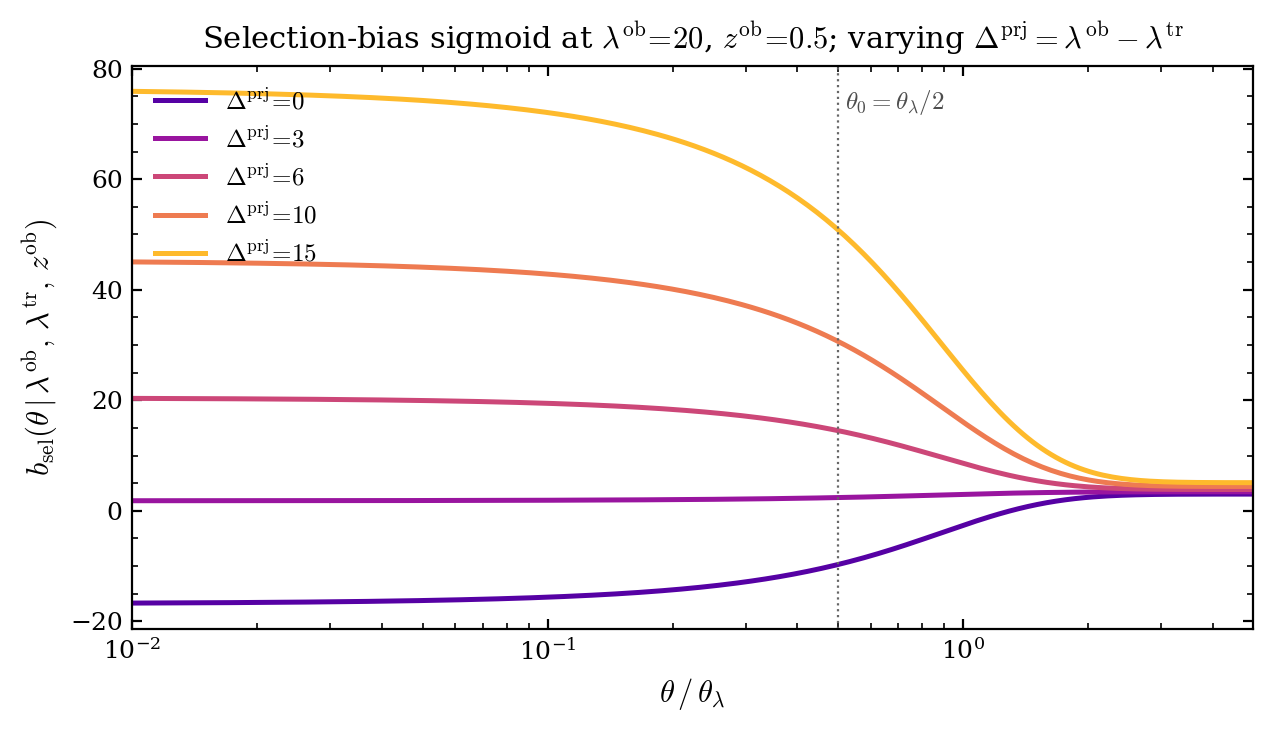
\includegraphics[width=0.92\textwidth]{figs/pedag_bsel_theta.png}
\caption{Selection-bias sigmoid
\(\bsel(\theta\,|\,\lob,\ltr,\zob)\) at fixed
\((\lob,\zob)=(20,0.5)\) as we vary the projection contamination
\(\dprj\equiv\lob-\ltr\). The \(x\)-axis is scaled by the per-bin
angle \(\theta_\lambda\), so the sigmoid pivot
\(\theta_0=\theta_\lambda/2\) (dotted) is universal. The
\(\theta\)-shape is fixed by the ansatz; \(\dprj\) drives both
plateaus through Steps~4--5. The left plateau \(\bsmall\) (close
neighbours projecting into the target aperture) grows fastest
with \(\dprj\); the right plateau \(\blarge\) (correlated
large-scale structure) moves less because it is closed by the
empirical \(\bhalo[1+0.13\,\delta^{\rm prj}]\) relation.}
\label{fig:pedag_bsel}
\end{figure}

\subsection{Projection kernel and \(\Pop[X]\) operator}

The \emph{projection kernel} \(\rhoprj\) is the per-halo weight
with which a projected halo at \((\lambda,z,\theta)\) contaminates
the observed richness of a target at \((\lob,\zob)\)
(\citealt{Costanzi2026}, eq.~\texttt{weight}):
\begin{equation}
\rhoprj(\lambda,z,\theta\mid\lob,\zob)
\;=\; w_z(z,\zob)\,f_A(\theta,\lob,\zob,\lambda,z)\,\lambda\,
      \mathbf{1}_{\{\lambda<\lob\}}.
\label{eq:rho_prj}
\end{equation}
Here \(\lambda\) is the projected halo's true richness;
\(z\) is its redshift; \(\theta\) is its angular separation from
the target; \(w_z(z,\zob)\) is the parabolic photo-\(z\) kernel
quantifying the probability that a galaxy at redshift \(z\) is
counted in the target's aperture at \(\zob\);
\(f_A(\theta,\lob,\zob,\lambda,z)\in[0,1]\) is the closed-form
overlap fraction of the two \textsc{redMaPPer} disks (of the
target and the projected halo); the factor \(\lambda\) converts
``this halo is present'' into ``this halo contributes \(\lambda\)
counts''; and the indicator
\(\mathbf{1}_{\{\lambda<\lob\}}\) implements the
\textsc{redMaPPer} ranking cut (only projected halos of lower
richness than the target contaminate the target's aperture).

The \emph{\(\Pop[X]\) operator} is the line-of-sight-averaged
integral of an arbitrary \(X(M,z,\theta)\) weighted by the halo
distribution and \(\rhoprj\):
\begin{align}
\Pop[X](\lob,\zob)
\;\equiv\;&
\int\!dz\,\frac{dV}{dz\,d\Omega}(z)\!
\int\!dM\,n(M,z)\!
\int\!d\lambda\,P(\lambda\mid M,z)
\notag\\
&\quad\cdot\;2\pi\int\!d\theta\,\sin\theta\;
\rhoprj(\lambda,z,\theta\mid\lob,\zob)\,X(M,z,\theta\mid\zob).
\label{eq:Pop}
\end{align}
The integrations marginalise, in order, over the projected halo's
redshift \(z\) (weighted by comoving volume per steradian
\(dV/dz\,d\Omega\)), mass \(M\) (weighted by the halo mass function
\(n(M,z)\)), true richness \(\lambda\) (weighted by the MOR
\(P(\lambda\mid M,z)\)), and angular separation \(\theta\) from the
target (with the usual \(2\pi\sin\theta\,d\theta\) sky-element).

Three specialisations drive the pipeline:
\begin{align}
\Pop[1]   &\;=\; \avg{\dprj_{\rm bkg}}(\lob,\zob),
&I_2 &\;\equiv\; \Pop\!\left[b\,\xinl\right],
&I_1 &\;\equiv\; \Pop\!\left[b\,\xinl\,\sigma(\theta)\right],
\end{align}
where \(b=b(M,z)\) is the Tinker-2010 halo bias (the halo's own
clustering amplitude) and
\(\xinl=\xinl(z,\zob,\theta)\) is the nonlinear matter correlation
function evaluated at the 3-D comoving separation
\(\Delta\chi(z,\zob,\theta)\) between the target at \(\zob\) and
the projected halo at \((z,\theta)\). By linearity,
\(\Pop[b\,\xinl(1-\sigma)] = I_2 - I_1\). Halo exclusion sets
\(\xinl\!\equiv\!0\) whenever \(\Delta\chi<R_{\rm excl}\).

\subsection{Bias pipeline}
\label{sec:pipeline}

This subsection gives the calculation chain from halo and
projection ingredients to the selection-affected cluster bias
\(\bsel(\lob,\zob,\theta)\) that
eq.~\eqref{eq:Sprj} requires. From the halo
ingredients \(\{n(M,z), b(M,z), P(\lambda\mid M,z)\}\) and the
projection ingredients \(\{w_z, f_A, \xinl\}\) it first evaluates
the halo-bias aggregate \(\bhalo(\lob,\zob)\) of
eq.~\eqref{eq:bhalo}, a 1-D \(\ln M\) integral at fixed \(\zob\).
In parallel, the hardest numerical block computes the three
forward integrals \(\Pop[1]\), \(I_1\), \(I_2\) of
eq.~\eqref{eq:Pop}; the recipes for this step are the subject of
\S\ref{sec:theta_split}--\ref{sec:zgrid} below. With these in hand, the random-aperture
projection contamination
\begin{equation}
\dprj_{\rm RND}(\lob,\zob) \;=\; \Pop[1](\lob,\zob)
                              + \bhalo(\lob,\zob)\,I_2(\lob,\zob)
\label{eq:dprj_rnd}
\end{equation}
follows by substituting \(\bsel\!\to\!\bhalo\) in the
\(\bsel\)-linearised identity (\(\bhalo\) pulls out of the mass
integral because it is mass-independent). The large-\(\theta\)
plateau is then
\begin{equation}
\blarge(\lob,\ltr,\zob) \;=\; \bhalo(\lob,\zob)\,
  \bigl[\,1 + 0.13\,\delta^{\rm prj}(\lob,\ltr,\zob)\,\bigr],
\qquad
\delta^{\rm prj} \;\equiv\; \frac{\lob-\ltr}{\dprj_{\rm RND}} - 1,
\label{eq:b_infty}
\end{equation}
where \(\delta^{\rm prj}\) is the fractional excess contamination
at \((\lob,\ltr,\zob)\) relative to a random aperture and the
empirical coefficient \(0.13\) is the Buzzard calibration. Finally
the small-\(\theta\) plateau closes the remaining linear equation
in \(\bsel\):
\begin{equation}
\bsmall(\lob,\ltr,\zob) \;=\;
\frac{(\lob-\ltr) - \Pop[1] - \blarge\,I_1}{I_2 - I_1},
\label{eq:b_small}
\end{equation}
where the denominator \(I_2-I_1 = \Pop[b\,\xinl(1-\sigma)]\) is the
contribution of the \(1-\sigma\) (small-\(\theta\)) part of the
sigmoid ansatz, and the numerator is what remains of the
\(\dprj\) identity once the \(\Pop[1]\) constant and the
\(\blarge\)-weighted \(I_1\) piece have been subtracted. With
\(\bsmall\) and \(\blarge\) both known, eq.~\eqref{eq:b_sigmoid}
returns \(\bsel(\lob,\ltr,\zob,\theta)\). Marginalising over
\(\ltr\) via
\begin{equation}
\bsel(\lob,\zob,\theta) \;=\;
\int\!d\ltr\;\bsel(\lob,\ltr,\zob,\theta)\,
P(\ltr\mid\lob,\zob),
\label{eq:b_marg_lt}
\end{equation}
with \(P(\ltr\mid\lob,\zob)\propto P(\lob\mid\ltr,\zob)\,
\pi(\ltr,\zob)\) and
\(\pi(\ltr,\zob) = \int dM\,n(M,z)\,P(\ltr\mid M,z)\) the prior on
the true richness, gives the final input to
eq.~\eqref{eq:Sprj}.

In \texttt{SelBias} (\S\ref{part:api}), steps computed once per
\((\lob,\zob)\) (\(\bhalo\), \(\Pop[1]\), \(I_1\), \(I_2\),
\(\dprj_{\rm RND}\)) are cached inside
\texttt{bias\_precompute}; the per-\(\ltr\) closures of
eqs.~\eqref{eq:b_infty}--\eqref{eq:b_small} live in
\texttt{bias\_from\_precomp}; and the sigmoid assembly +
\(\ltr\)-marginalisation are \texttt{b\_lob\_theta} and
\texttt{b\_sel\_marginalised} respectively.

\subsection{Two-halo projected profile}
\label{sec:Sprj}

\citet{Costanzi2026}, eq.~\texttt{sigprj}:
\begin{multline}
\avg{\Sprj(R\mid\lob,\zob)} =
\int\!d\theta\,\sin\theta\int\!dz\,\frac{dV}{dz\,d\Omega}\int\!dM\,n(M,z) \\
\cdot\bigl[\,1 + b(M,z)\,\bsel(\lob,\zob,\theta)\,\xinl(z,\zob,\theta)\bigr]\,
  \Smis(R\mid M,z,\theta,\zob).
\label{eq:Sprj}
\end{multline}
Here \(R\) is the physical projected distance around the target
in \(\hMpc\); \(\theta\) is the angular separation of the
contaminating halo from the target; \(z\) is the halo's redshift;
\(M\) its mass; \(n(M,z)\) the halo mass function; \(b(M,z)\) the
halo bias; \(\bsel\) the selection-affected cluster bias from
eq.~\eqref{eq:b_marg_lt}; \(\xinl\) the nonlinear matter
correlation function at the 3-D separation between the target and
the \((z,\theta)\) halo; and \(\Smis\) is the azimuth-averaged
miscentered NFW surface density. The \(1\) inside the bracket is
the mean (uncorrelated) contribution; the \(b\,\bsel\,\xinl\) term
is the correlation-function boost that the two-halo term
captures.

\(\Smis\) is the one-halo surface density integrated over the
azimuthal angle \(\varphi\) because the projected halo is
off-centre with respect to the profile radius:
\begin{equation}
\Smis(R\mid M,z,\theta,\zob) =
\int_0^{2\pi}\!d\varphi\;\Sigma(R_h\mid M,z),
\qquad
R_h = \sqrt{R^2 + R_\theta^2 - 2 R R_\theta \cos\varphi},
\label{eq:Smis}
\end{equation}
with \(R_\theta \equiv \theta\,D_A(\zob)\) the physical projected
distance from the target to the contaminating halo and
\(\Sigma(R_h\mid M,z)\) the centred NFW surface density of the
contaminating halo at 2-D radius \(R_h\) from its own centre.
\(\Smis\) is tabulated from the offset-NFW lookup
(\texttt{nfw.py}), with a factor of 2 to match the
\(\int_0^{2\pi}\) convention.

\begin{figure}[!htbp]
\centering
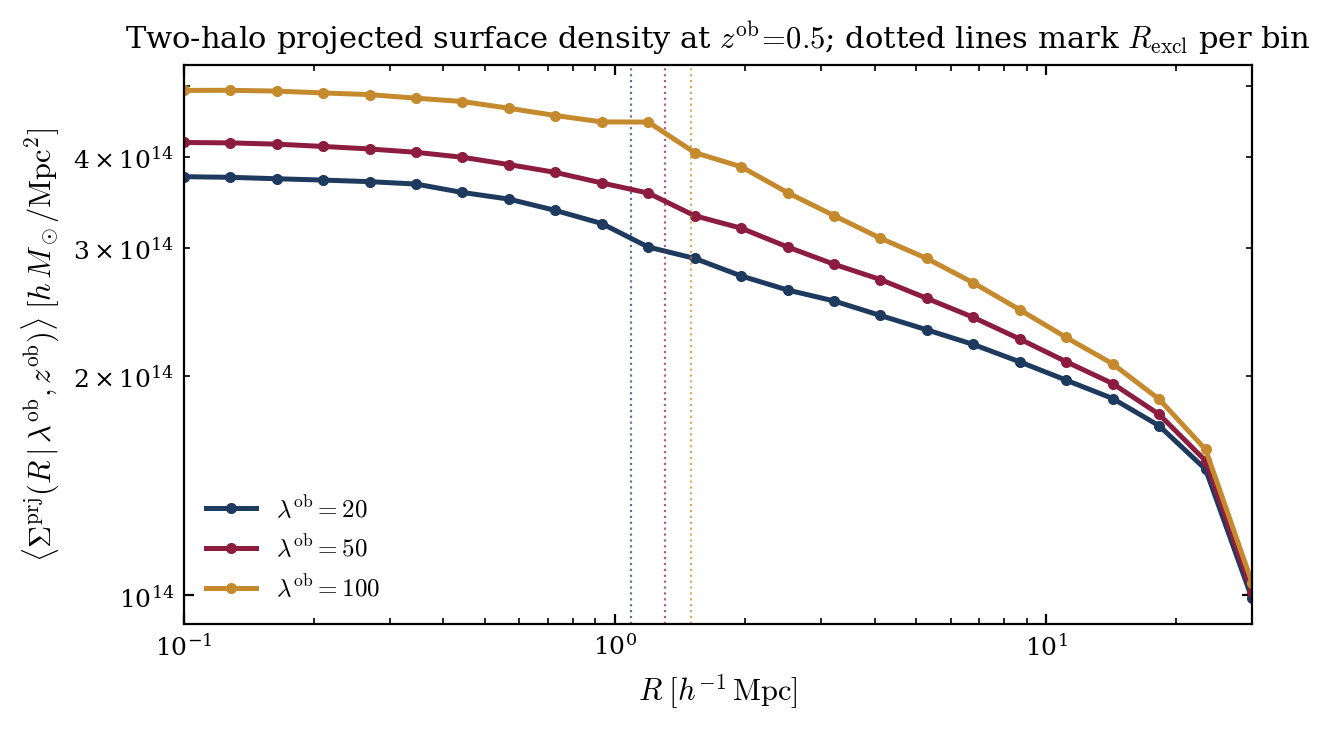
\includegraphics[width=0.92\textwidth]{figs/pedag_sigma_prj.png}
\caption{Two-halo \(\avg{\Sprj(R\,|\,\lob,\zob)}\) at
\(\zob=0.5\), three richness bins. Dotted lines mark the per-bin
exclusion scale \(R_{\rm excl}=R_\lambda(\lob)(1+\zob)\), which
separates the miscentered-NFW-dominated inner regime from the
correlated \(\bsel\!\cdot\!\xinl\) large-scale regime.}
\label{fig:pedag_sigmaprj}
\end{figure}

\begin{figure}[!htbp]
\centering
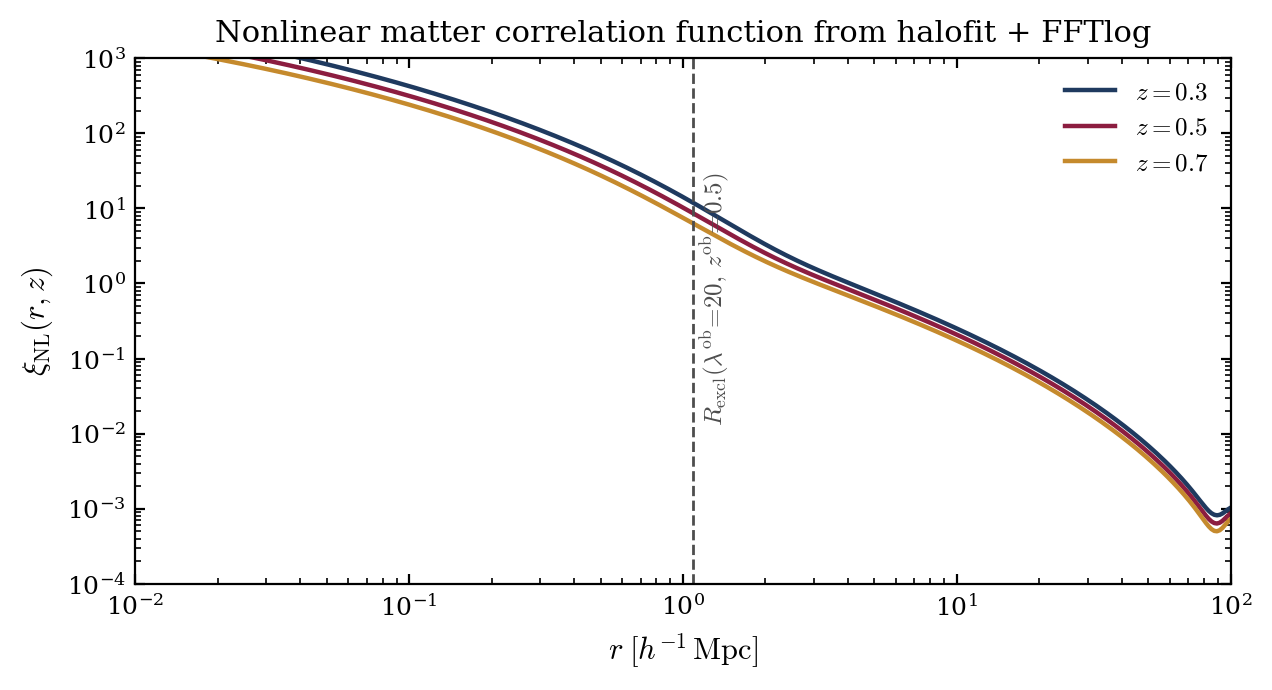
\includegraphics[width=0.82\textwidth]{figs/pedag_xi_nl.png}
\caption{Nonlinear matter correlation function \(\xinl(r,z)\) from
halofit + FFTlog (\texttt{xi\_nl.py}). Dashed line: \(R_{\rm excl}\)
at the reference point \((\lob,\zob)=(20,0.5)\). The near-power-law
\(\xinl\propto r^{-1.7}\) between \(\sim 0.1\) and
\(\sim 5\,\hMpc\) drives the exclusion-peak structure of the
\(z\)-integrand in \S\ref{sec:fz_structure}.}
\label{fig:pedag_xinl}
\end{figure}

\section*{\textcolor{harvardcrimson}{Numerical pitfalls}}
\addcontentsline{toc}{section}{Numerical pitfalls}

The three forward integrals that carry the whole pipeline ---
\(\Pop[1]\), \(I_1\), \(I_2\) of eq.~\eqref{eq:Pop} --- are 4-D
integrals over \((z,\,\theta,\,M,\,\lambda)\). The inner
\((M,\lambda)\) axes are well-behaved and a plain
Gauss--Legendre (GL) rule with \(N_M\!=\!24\) and
\(N_\lambda\!=\!60\) converges them to \(<\!10^{-4}\); that part
of the integration is boring. The outer \((z,\theta)\) axes,
however, contain two sharp, physics-driven features that punish
any uninformed fixed-rule method and were the source of the
largest precision bugs we saw while developing this package:

\begin{itemize}
  \item the \textbf{halo-exclusion step in \(\theta\)}: at each
        \(z\) the integrand has a hard discontinuity at
        \(\theta=\theta_{\rm excl}(z)\), where \(\xinl\) is set
        to zero by the exclusion prescription. A fixed GL grid on
        \((0,2\theta_\lambda)\) with a mask integrates across this
        step and stalls at \(\sim 0.3\%\) error regardless of
        \(N_\theta\) (\S\ref{sec:theta_split});
  \item the \textbf{exclusion-peak + ring-plateau structure in
        \(z\)}: the photo-\(z\) kernel carves out a window of
        width \(\sim\!0.1\) around \(\zob\), and inside that
        window \(\xinl\) produces twin sharp peaks at
        \(z=\zob\!\pm\!\delta z_{\rm excl}\) sitting on top of a
        narrow plateau --- three qualitatively different regions
        crammed into \(|z-\zob|\!\lesssim\!5\!\times\!10^{-4}\)
        (\S\ref{sec:zgrid}).
\end{itemize}

The recipes below move the GL nodes onto the physically correct
coordinate in each region so that \emph{the sharp features land
at grid boundaries}, where GL rules naturally cluster nodes. The
result is sub-\(0.01\%\) precision on all three integrals at
\(N_z\!=\!80\), \(N_\theta\!=\!10\) vs
\texttt{scipy.integrate.quad} with matched inner grids. Total cost
at \((\lob,\zob)=(20,0.5)\): \(\sim 26\) ms per
\texttt{SelBias.bias\_precompute}. If the bullets below already
look familiar, the executive-summary version is: split the
\(\theta\)-axis at the exclusion boundary (per-\(z\) GL on
\([\theta_{\rm excl}(z),\,2\theta_\lambda]\), no mask); split the
\(z\)-axis by physics into a ring band + two outer halves,
integrating in \(z\) on the ring and in
\(u=\ln|\Delta\chi_\parallel|\) on the outers.

\section{\texorpdfstring{The \(\theta\)-axis: split at exclusion}{The theta-axis: split at exclusion}}
\label{sec:theta_split}

\paragraph{What this section fixes.}
The \(\theta\)-axis of \(\Pop[1], I_1, I_2\) runs over the angular
separation between the target and each projected halo. Halo
exclusion makes this a discontinuous integrand, which breaks any
fixed GL rule that sees the discontinuity as a noisy feature. Below
we show why that happens and how moving the lower integration
limit onto the discontinuity turns the problem into a smooth
integral whose GL convergence is at its design rate.

At any \(z\), halo exclusion kills \(\theta\) below a threshold
\(\theta_{\rm excl}(z)\) obtained from
\(\Delta\chi(z,\theta_{\rm excl})=R_{\rm excl}\):
\begin{equation}
\cos\theta_{\rm excl}(z)
= \frac{\chi(z)^2+\chi(\zob)^2-R_{\rm excl}^2}{2\,\chi(z)\,\chi(\zob)},
\qquad \text{clipped to }[-1,1].
\label{eq:theta_excl_def}
\end{equation}

A fixed-grid \(N_\theta\!=\!20\) GL on \((0,2\theta_\lambda)\) with
\(\xinl\!\to\!0\) inside the step integrates across a
discontinuity: the error oscillates in \(N_\theta\) and settles to
a \(\sim 0.3\%\) floor. The fix is a per-\(z\) change of the
integration interval: when \(\theta_{\rm excl}(z)>0\), integrate on
\([\theta_{\rm excl}(z),\,2\theta_\lambda]\) with no mask. GL
nodes cluster at the endpoints where the step sits; the integrand
is smooth on the interval.
\begin{center}
\small
\begin{tabular}{r r r r}
\toprule
\(N_\theta\) & \(\Pop[1]\) err & \(I_2\) err & \(I_1\) err \\
\midrule
5   & \(+0.060\%\) & \(+0.046\%\) & \(+0.046\%\) \\
\textbf{10}  & \(\mathbf{-0.005\%}\) & \(\mathbf{-0.001\%}\) & \(\mathbf{-0.004\%}\) \\
15  & \(+0.000\%\) & \(+0.000\%\) & \(+0.000\%\) \\
\bottomrule
\end{tabular}
\end{center}
\(N_\theta=10\) reaches sub-\(0.01\%\): \(\sim 12\times\) node
reduction and two decades better precision than the mask recipe.

\section{\texorpdfstring{The \(z\)-axis: split by physics}{The z-axis: split by physics}}
\label{sec:zgrid}

\paragraph{What this section fixes.}
With \(\theta\) handled, the outer \(z\)-integral becomes the
dominant source of residual error --- not because it is hard in
absolute terms, but because its integrand has three different
shapes over a \(\sim\!10^{-3}\)-wide window around \(\zob\). A
single uniform \(z\)-grid under-samples the exclusion peaks; a
single log-spaced grid in \(|\Delta\chi_\parallel|\)
over-concentrates on the inner edge and misses the ring plateau.
The fix is to integrate each physical region on the coordinate in
which \emph{that} region is smooth, and stitch them together.

Each of \(\Pop[1], I_1, I_2\) factorises into an outer
\(z\)-integral times an \emph{inner} \((M,\lambda,\theta)\)-integral,
\begin{equation}
I \;=\; \int\!dz\;f_X(z),
\qquad
f_X(z)\;\equiv\;\frac{dV}{dz\,d\Omega}(z)\,w_z(z,\zob)\,
\mathcal{I}_{\rm inner}^{X}(z),
\label{eq:fz_def}
\end{equation}
where the inner integral is the full \((M,\lambda,\theta)\) block
of eq.~\eqref{eq:Pop} evaluated at a single \(z\),
\begin{equation}
\mathcal{I}_{\rm inner}^{X}(z)
\;\equiv\;
\int\!dM\,n(M,z)\!
\int\!d\lambda\,P(\lambda\mid M,z)\,\lambda\,
\mathbf{1}_{\{\lambda<\lob\}}
\cdot 2\pi\!\int\!d\theta\,\sin\theta\;
f_A(\theta,\lob,\zob,\lambda,z)\,X(M,z,\theta\mid\zob),
\label{eq:Iinner}
\end{equation}
and \(X\) is the per-operator integrand label:
\(X\!=\!1\) for \(\Pop[1]\),
\(X\!=\!b(M,z)\,\xinl(z,\zob,\theta)\) for \(I_2\), and
\(X\!=\!b(M,z)\,\xinl(z,\zob,\theta)\,\sigma(\theta)\) for \(I_1\).
\(f_X(z)\) is therefore the \(z\)-density that the outer integral
has to quadrature.

For \(\Pop[1]\), \(X\!=\!1\) contains no \(\xinl\) and no
exclusion; \(f_{\Pop[1]}(z)\) is a smooth single-peaked function
of width \(\sim\sigma_z(\zob)\) peaked at \(z\!=\!\zob\)
(Fig.~\ref{fig:fz} left panel, dashed blue curve). For \(I_1,
I_2\) the halo-exclusion cut carves three regions. Defining
\(\delta z_{\rm excl}\equiv R_{\rm excl}/(c/H(\zob))\) (at the
reference point, \(\approx 4.7\times 10^{-4}\)):
\begin{enumerate}
  \item \emph{Ring plateau} \(|z-\zob|<\delta z_{\rm excl}\): the
        small-\(\theta\) part is excluded; only
        \(\theta>R_{\rm excl}/\chi(\zob)\) contributes through a
        ring of structure at \(\Delta\chi>R_{\rm excl}\). Visible
        as a flat core of \(f_{I_2}(z)\) between the dotted lines
        in Fig.~\ref{fig:fz} right panel.
  \item \emph{Exclusion peaks} at
        \(|z-\zob|\!\approx\!\delta z_{\rm excl}\): \(\xinl\) is
        evaluated at \(\Delta\chi\!\to\!R_{\rm excl}\), its largest
        resolved value. \(f_{I_2}(z)\) has two sharp peaks at
        \(z=\zob\pm\delta z_{\rm excl}\), a few times the plateau
        amplitude (Fig.~\ref{fig:fz} right panel).
  \item \emph{Outer decay}:
        \(f(z)\!\propto\!\Delta\chi_\parallel^{-1.7}\) modulated
        by \(w_z\), truncating at
        \(|z-\zob|\!\sim\!\sigma_z(\zob)\!\approx\!0.09\)
        (Fig.~\ref{fig:fz} left panel, outer wings).
\end{enumerate}

\begin{figure}[!htbp]
\centering
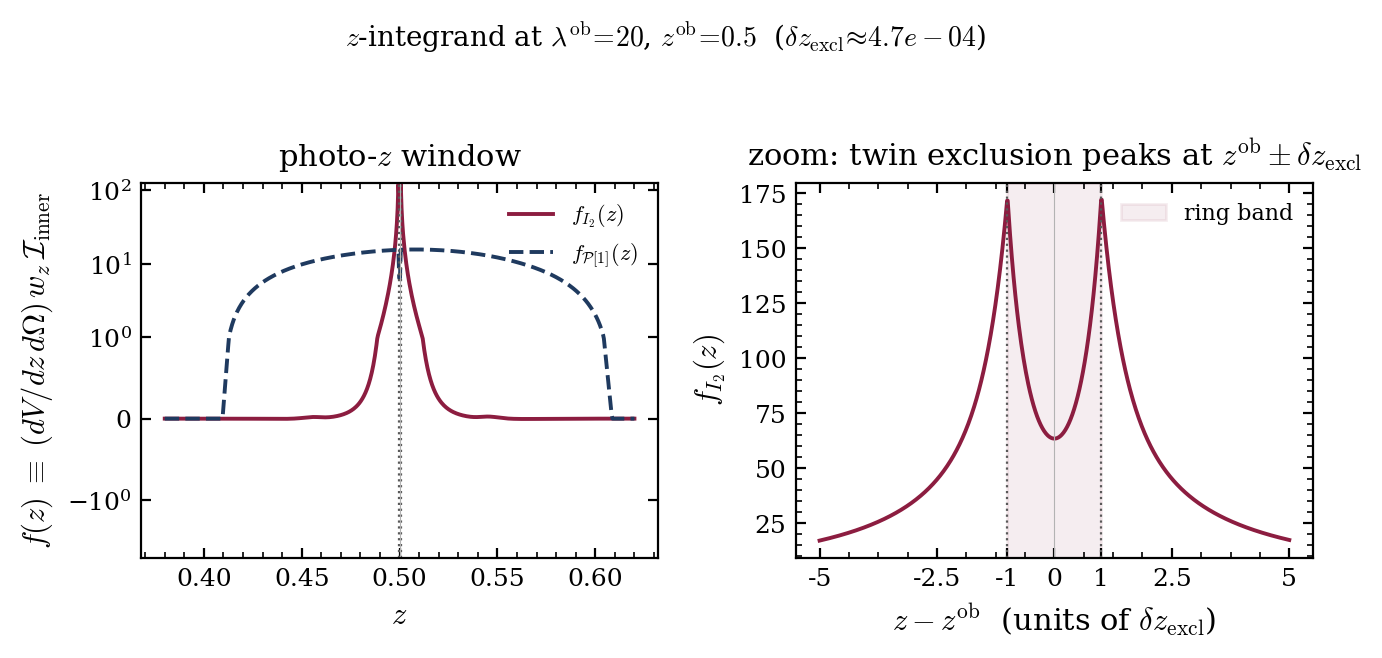
\includegraphics[width=\textwidth]{figs/pedag_fz_integrand.png}
\caption{The \(z\)-integrand \(f_X(z)\) of eq.~\eqref{eq:fz_def}
at \((\lob,\zob)=(20,0.5)\). \emph{Left:} full photo-\(z\)
window, symlog \(y\)-scale; the red solid curve is
\(f_{I_2}(z)\), the blue dashed curve is \(f_{\Pop[1]}(z)\).
\(\Pop[1]\) (no \(\xinl\)) is smooth and single-peaked;
\(I_2\) has an additional two-peak exclusion substructure at
\(z^{\rm ob}\!\pm\!\delta z_{\rm excl}\) (dotted vertical lines)
that is invisible at this scale but inflated by the symlog
axis. \emph{Right:} zoom to
\(|z-z^{\rm ob}|<5\,\delta z_{\rm excl}\), linear scale. The
twin exclusion peaks are resolved; the ring-plateau band between
them (red shading) is where \(\xinl\) is excluded and the
integrand is flat. A naive uniform \(z\)-grid places zero nodes
inside this window and under-samples both peaks, which is the
hazard the split-by-physics recipe avoids.}
\label{fig:fz}
\end{figure}

Write \(I = I_{\rm ring} + I_{\rm outer}^{\rm fg}
+ I_{\rm outer}^{\rm bg}\) and integrate each region on a grid
tailored to its shape. The ring band
\((\zob-\delta z_{\rm excl},\zob+\delta z_{\rm excl})\) uses GL in
\(z\) (smooth integrand, \(N_{\rm ring}\!=\!\max(9,\,N_z/4)\)). The
outer pieces use GL in \(u=\ln|\Delta\chi_\parallel|\), so
\(\xinl\!\propto\!e^{-1.7u}\) peaks at the inner endpoint
\(u=\ln R_{\rm excl}\) where GL naturally clusters nodes. Per side:
\(N_{\rm outer}=\max(15,\,(N_z-N_{\rm ring})/2)\). Each region's
integrand is smooth in its own variable; the sharp features sit at
region boundaries where GL rules converge at their design rate.

At \(N_z\!=\!80\) this reaches sub-\(0.01\%\) on \(\Pop[1],I_1,I_2\)
vs \texttt{scipy.integrate.quad} with matched inner grids (regression
test \texttt{tests/test\_integrals.py::TestSelBiasThetaSplit}).
Edge cases (\(R_{\rm excl}\) exceeds the photo-\(z\) support, or
the ring band is wider than it) degrade gracefully via empty-array
guards.

\clearpage
\section*{\textcolor{harvardcrimson}{API and glossary}}
\addcontentsline{toc}{section}{API and glossary}
\label{part:api}

This section is a pointer table from the math above to the code
that computes each quantity. The glossary table lists every
symbol with its defining equation, a one-line description, and
the Python call that returns it.

\section{Objects}

\paragraph{\texttt{Cosmology}} (\texttt{cosmology.py}).
Flat-\(\Lambda\)CDM background. Provides
\texttt{chi(z)} \(=\chi(z)\) comoving distance,
\texttt{dV\_dzdOm(z)} \(= dV/dz\,d\Omega\), and \texttt{h}, \texttt{H0}.
Default: Buzzard-v1.1.

\paragraph{\texttt{PkGrid}} (\texttt{pk.py}).
CAMB-backed linear \(P(k,z)\). One CAMB call per cosmology;
re-evaluated in place for each \((k,z)\) request.

\paragraph{\texttt{SigmaM}} (\texttt{sigma\_m.py}).
\(\sigma(M,z)\) top-hat variance via a Simpson rule on
\texttt{PkGrid}'s \(k\)-grid. Used by both \texttt{HMF} and
\texttt{Bias}.

\paragraph{\texttt{HMF}} (\texttt{hmf.py}).
Tinker 2008, \(\Delta=200\). \texttt{hmf(M, z)} returns
\(n(M,z)\) in \(\hMsun^{-1}\,\hMpc^{-3}\).

\paragraph{\texttt{Bias}} (\texttt{bias.py}).
Tinker 2010 peak-height halo bias. \texttt{bias(M, z)} returns
\(b(M,z)\).

\paragraph{\texttt{MOR}} (\texttt{mor.py}).
Mass--observable relation. \texttt{mor.pdf(lam, M, z)} returns
\(P(\lambda\mid M,z)\), the EMG kernel of Costanzi 2019.

\paragraph{\texttt{XiNL}} (\texttt{xi\_nl.py}).
Nonlinear matter correlation function \(\xinl(r,z)\) from halofit
\(P_{\rm NL}\) via an FFTlog Hankel transform. Lazy build
(first call pays \(\sim 2\) s, cached thereafter).

\paragraph{\texttt{SelBias}} (\texttt{sel\_bias.py}).
The bias pipeline (\S\ref{sec:pipeline}). Holds references to all
of the above. See the glossary below for per-method meanings.

\paragraph{\texttt{NFWMiscentered}} (\texttt{nfw.py}).
\(\Smis(R\mid M,z,\theta,\zob)\) from the three offset-NFW lookup
tables (Costanzi-notebook convention).

\paragraph{\texttt{SigmaPrj}} (\texttt{sigma\_prj.py}).
The \(\avg{\Sprj}\) orchestrator (eq.~\ref{eq:Sprj}).
\texttt{SigmaPrj(cosmo, sel\_bias, nfw)(R, lob, zob)} returns
\(\avg{\Sprj(R)}\).

\paragraph{\texttt{GridConfig}} (\texttt{config.py}).
Grid-size defaults: \(N_z\!=\!80\), \(N_\theta\!=\!10\),
\(N_M\!=\!24\). \(N_\lambda\) is a separate \texttt{SelBias}
constructor arg (default 60).

\section{Glossary of quantities}
\label{sec:glossary}

Rows group by role: halo ingredients, projection ingredients, the
\(\Pop\) operator specialisations, the bias-pipeline outputs, and
the profile. ``Eq.'' links to the defining equation; ``Code''
gives the Python call.

\renewcommand{\arraystretch}{1.25}
\begin{center}
\small
\begin{tabular}{@{}p{0.20\textwidth} p{0.36\textwidth} c p{0.32\textwidth}@{}}
\toprule
\textbf{Symbol} & \textbf{Meaning} & \textbf{Eq.} & \textbf{Code} \\
\midrule
\multicolumn{4}{@{}l}{\emph{Halo ingredients}} \\
\midrule
\(n(M,z)\) & Tinker-2008 halo mass function (\(\Delta\!=\!200\)) &
  \eqref{eq:bhalo} & \texttt{HMF(sigma\_m)(M, z)} \\
\(b(M,z)\) & Tinker-2010 peak-height halo bias &
  \eqref{eq:bhalo} & \texttt{Bias(sigma\_m)(M, z)} \\
\(P(\lambda\mid M,z)\) & MOR kernel (Costanzi-2019 EMG) &
  \eqref{eq:Pop} & \texttt{MOR().pdf(lam, M, z)} \\
\(\xinl(r,z)\) & Nonlinear matter 2pt correlation (halofit+FFTlog); zero below \(R_{\rm excl}\) &
  \eqref{eq:Pop} & \texttt{XiNL(cosmo)(r, z)} \\
\midrule
\multicolumn{4}{@{}l}{\emph{Projection kernel and \(\Pop[X]\) operator}} \\
\midrule
\(\rhoprj\) & Per-halo projection weight \(w_z\,f_A\,\lambda\,\mathbf{1}_{\{\lambda<\lob\}}\) &
  \eqref{eq:rho_prj} & internal to \texttt{SelBias.\_P\_operator} \\
\(\Pop[X]\) & LoS average of \(X\) weighted by \(\rhoprj\) and halo distribution &
  \eqref{eq:Pop} & \texttt{SelBias.\_P\_operator(lob, zob)} \\
\(\Pop[1]\equiv\avg{\dprj_{\rm bkg}}\) & Mean background projection (no \(\xinl\), smooth in \(z\)) &
  \eqref{eq:Pop} & \texttt{bias\_precompute(lob,zob)['P1']} \\
\(I_2\equiv\Pop[\,b\,\xinl\,]\) & Halo-bias-weighted \(\xinl\); drives \(\dprj_{\rm RND}\) &
  \eqref{eq:Pop} & \texttt{bias\_precompute(lob,zob)['I2']} \\
\(I_1\equiv\Pop[\,b\,\xinl\,\sigma(\theta)\,]\) & \(I_2\) weighted by the sigmoid; enters Step~5 &
  \eqref{eq:Pop} & \texttt{bias\_precompute(lob,zob)['I1']} \\
\midrule
\multicolumn{4}{@{}l}{\emph{Bias-pipeline outputs}} \\
\midrule
\(\bhalo(\lob,\zob)\) & Halo-bias aggregate at fixed \(\lob\) (paper's \(b_{\rm eff}\)) &
  \eqref{eq:bhalo} & \texttt{SelBias.b\_eff(lob, zob)} \\
\(\dprj_{\rm RND}\) & Projection contamination of a random aperture &
  \eqref{eq:dprj_rnd} & \texttt{bias\_precompute(lob,zob)['Delta\_RND']} \\
\(\blarge\) & Large-\(\theta\) plateau (empirical closure) &
  \eqref{eq:b_infty} & \texttt{bias\_from\_precomp(pre,ltr)['b\_infty']} \\
\(\bsmall\) & Small-\(\theta\) plateau (Step~5 inversion) &
  \eqref{eq:b_small} & \texttt{bias\_from\_precomp(pre,ltr)['b\_zero']} \\
\(\bsel(\lob,\ltr,\zob,\theta)\) & Scale-dependent bias via sigmoid ansatz &
  \eqref{eq:b_sigmoid} & \texttt{SelBias.b\_lob\_theta(th,ltr,zob,lob,precomp=pre)} \\
\(\bsel(\lob,\zob,\theta)\) & \(\ltr\)-marginalised bias; input to \(\avg{\Sprj}\) &
  \eqref{eq:b_marg_lt} & \texttt{SelBias.b\_sel\_marginalised(th,lob,zob,precomp=pre)} \\
\midrule
\multicolumn{4}{@{}l}{\emph{Two-halo profile}} \\
\midrule
\(\Smis(R\mid M,z,\theta,\zob)\) & Azimuth-averaged miscentered NFW (offset-NFW lookup) &
  \eqref{eq:Smis} & \texttt{NFWMiscentered(cosmo).sigma\_grid(R,Rtheta,M,z)} \\
\(\avg{\Sprj(R\mid\lob,\zob)}\) & Two-halo projected surface density (main output) &
  \eqref{eq:Sprj} & \texttt{SigmaPrj(cosmo,sel\_bias,nfw)(R,lob,zob)} \\
\bottomrule
\end{tabular}
\end{center}

\section{Validation}

\paragraph{Unit tests.} \texttt{tests/test\_integrals.py}:
\texttt{TestSelBiasThetaSplit} (sub-\(0.1\%\) vs quad at
\(N_\theta\!=\!10\)), \texttt{TestLambdaAxisConverged} (\(n_\ltr\!=\!30\)
matches \(100\) to \(<\!10^{-4}\)), \texttt{TestSigmaPrjTheta}
(split-at-\(\theta_R\) + monotonicity). \texttt{test\_smoke.py}:
end-to-end smoke test.

\paragraph{Validation scripts.} \texttt{validations/}:
\texttt{theta\_convergence.py} sweeps \(N_\theta\);
\texttt{quad\_matched\_inner.py} compares the
\texttt{\_P\_operator} output to \texttt{scipy.integrate.quad}
with matched inner GL grids;
\texttt{quad\_validate.py} is the end-to-end quad cross-check.

\paragraph{Defaults.} \(N_z\!=\!80\), \(N_\theta\!=\!10\),
\(N_M\!=\!24\), \(N_\lambda\!=\!60\). No retuning is needed across
the Y3 range \((\lob\!\in\![20,500],\,\zob\!\in\![0.1,0.8])\):
only \(R_{\rm excl}\) and \(c/H(\zob)\) shift, and both are tracked
analytically by the grid builder.

\bibliographystyle{plainnat}
\begin{thebibliography}{}
\bibitem[Costanzi et al.(2026)]{Costanzi2026}
Costanzi, M., Wu, H.-Y., Esteves, J.~H., Grandis, S., To, C., \&
Aguena, M.\ 2026, Phys.~Rev.~D (accepted), arXiv:2604.05833.
\end{thebibliography}

\end{document}
